% Chapter 6

\chapter{Farben} % Main chapter title

\label{Farben} % For referencing the chapter elsewhere, use \ref{Chapter1}

\lhead{\chaptername{} \thechapter{} - \emph{Farben}} % This is for the header on each page - perhaps a shortened title

%----------------------------------------------------------------------------------------

Neben der Typographie stellten sich die Farben als eines der komplexesten Themengebiete heraus. Viele Entscheidungen im Bezug auf Farben müssen auf einer subjektiven Ebene getroffen werden, einige können jedoch, zumindest bedingt, durch Regeln beschrieben werden.

Dieses Kapitel beschäftigt sich mit verschiedenen Fragestellungen. Zunächst wird der Versuch unternommen, herauszufinden, ob die Verwendung bestimmter Farben immer empfohlen oder von dessen Verwendung abgeraten werden kann.
Weiterhin wird versucht, Regeln für die Kombination von verschiedenen Farben zu finden. Die Frage, wie und in welchem Umfang Farben in einer Gestaltung eingesetzt werden sollten, wird beantwortet und es wird der Versuch unternommen, einen Workflow zum Finden von Farben zu definieren. Außerdem wird die Verwendung von Farben auf den nativen Plattformen Android und iOS behandelt.

%----------------------------------------------------------------------------------------

\section{Farbwirkung}

Um herauszufinden, ob bestimmte Farben empfohlen oder von ihnen abgeraten werden kann, soll hier zunächst der psychologische Effekt von Farben auf Menschen behandelt werden.

Zunächst lässt sich feststellen, dass Farben eine Wirkung auf die menschliche Wahrnehmung und ihr Verhalten haben. In den letzten drei Jahren konnte beispielsweise während des Moduls \textit{Grundlagen der visuellen Kommunikation} beobachtet werden, wie ein Raum von über 100 Menschen fast einstimmig bestimmte Farbkombinationen mit Adjektiven belegten. Auch in der Forschung wir diese Annahme unterstützt:

\begin{quote}
Color filters humanity’s perception of the world and alters people’s relationships with their surroundings. It influences human perception, preference, and psychology throughout the lifespan. \cite{rider2010color}
\end{quote}

\begin{quote}
Colour has the potential to elicit emotions or behaviors [...] \cite{cyr2010colour}
\end{quote}

Die Frage, die es zu beantworten gilt, lautet also nicht, ob es möglich ist Menschen mit Farben zu beeinflussen, sondern vielmehr \textit{wie}. Konkret sollte untersucht werden, ob es bestimmte Farben gibt, die bei einem Großteil der Menschen positive bzw. negative Gefühle hervorrufen, um so eine solide Basis für das Erstellen eines Farbschemas zu schaffen.

%----------------------------------------------------------------------------------------

\section{Beliebtheit von Farben}

Generell lässt sich keine absolute und allgemeingültige Regel aufstellen, welche Farben am beliebtesten sind. Dies hängt von verschiedenen Faktoren wie, Herkunft, Kultur, Geschlecht und Charakterausprägung des Individuums ab. Für Westeuropäische Erwachsene weist aber die von \cite{eysenck1941critical} erstellte Hierarchie \textit{Blau, Rot, Grün, Violett, Orange, Gelb} eine hohe Gültigkeit auf. \\
Es lässt sich aber auch feststellen, dass kalte Farbtöne beliebter sind als warme, was wiederum (zumindest in Teilen) im Widerspruch mit der oben aufgestellten Hierarchie steht. 
Zwar läge die Möglichkeit nahe, wegen seiner Beliebtheit immer Blau als Grundfarbe zu empfehlen, jedoch soll hier im weitern Verlauf überprüft werden, ob auch andere (vielleicht konkretere) Grundlagen für eine Farbempfehlung gefunden werden können. \\
Zumindest konnte hier aber ein erster Ansatzpunkt für die Verwendung von Farben gefunden werden.


%----------------------------------------------------------------------------------------

\section{Psychologische Wirkung von Farben}

Eine dieser Möglichkeiten stellt die Auswahl der Farbe nach einem intendierten Effekt auf den Betrachter dar.
Hier unterscheiden sich sowohl Farbtöne, als auch einzelne Farben.
So erhöhen warme Farbtöne, wie Rot und Gelb, den Puls und verursachen Hunger beim Betrachter \cite{berman2010street},
bei einigen kalten Farbtönen, wie zum Beispiel Blau, kann hingegen ein ein beruhigender Effekt auf den Betrachter nachgewiesen werden \cite{crozier1999meanings}.

\cite{berman2010street} listet einige der beliebtesten Farben samt ihrer Bedeutung auf. Die Bedeutungen gelten hierbei explizit für Nordamerika, sollten aber auch in der restlichen westlichen Welt eine ähnliche Gültigkeit aufweisen.

\textit{Rot} hat, je nach Kontext, verschiedene (und teilweise recht unterschiedliche) Bedeutungen. So gilt Rot als Farbe der Romantik, Liebe und Leidenschaft, wird jedoch auch als Signalfarbe auf Straßenschildern genutzt und kann in gewissen Kontexten als Zeichen für Gefahr stehen.

\textit{Gelb und Orange} rufen Erinnerungen an die Sonne hervor und gelten daher als fröhliche Farben, sind im allgemeinen aber eher unbeliebt. Gelb ist oft heller als Weiß und wird als Signalfarbe genutzt, Orange erhöht ,ähnlich wie Rot, den Appetit des Betrachters.

\textit{Blau} ist in der westlichen Welt die beliebteste Farbe, ihr wird eine beruhigende Wirkung nachgesagt. In verschiedenen Abstufungen wirkt Blau jedoch verschieden, von dynamisch bis zuverlässig.

\textit{Grün} steht hauptsächlich als Farbe der Natur und der Gesundheit, kann in dunkleren Abstufungen aber auch für Wohlstand stehen.

\textit{Violett} steht für das Noble und Majestätische, kann gleichzeitig aber auch für Einsamkeit stehen.

Es ist also schwer, einer Farbe genau eine Eigenschaft zuzuschreiben, häufig hat die gleiche Farbe in einer helleren oder dunkleren Abstufung eine andere Wirkung. Zumindest lässt sich aber eine grobe Auflistung von Eigenschaften finden, auf dessen Basis eine Farbempfehlung erfolgen könnte.

Wie zu Anfang bereits vermutet, lässt sich für das Finden einer Grundfarbe also keine definitive Empfehlung abgeben, gerade auch weil es für die Verwendung von Farben auf dieser Ebene zunächst kein \textit{Richtig} oder \textit{Falsch} gibt. Es lassen sich mit der Beliebtheit und der psychologischen Wirkung aber zumindest Ansätze finden, auf dessen Basis dem Nutzer die Farbfindung erleichtert werden kann.

%----------------------------------------------------------------------------------------

\section{Kontraste und Farbschemata}

Für die Erstellung einer Farbpalette müssen im nächsten Schritt Farben miteinander kombiniert werden. Um diese Farben so zu kombinieren, dass sie zusammen ein harmonisches Bild ergeben, gibt es verschiedene Farbkontraste mit denen gearbeitet werden kann.
Hier sollen zunächst die verfügbaren Farbkontraste auf eine Verwendbarkeit im Tool und ihre programmatische Umsetzbarkeit hin untersucht werden.
Weiterhin werden einige bereits bestehende Tools zum Erstellen von Farbpaletten auf ihre Stärken und Schwächen untersucht.

\cite[S.22]{whelan1994color} beschreibt zehn grundlegende Farbschemata, von denen in diesem Projekt, mit Blick auf den Umfang und die Verwendung in tatsächlichen Projekten, nur drei von Bedeutung sein sollen: \textit{Komplementär, Monochromatisch} \textit{und Geteilt Komplementär (häufig auch Triadisch genannt)}.
Diese Farbschemata bestehen aus einer bis drei Farben (wobei \textit{Farben} hier im Sinne der Definition zu verstehen sind, Grautöne, Weiß und Schwarz also von der Zählung ausgenommen sind, obwohl auch sie in fast jedem Farbschema Verwendung finden).

Die Frage nach dem richtigen Farbschema für eine bestimmte Situation kann hier nicht beantwortet werden, jedoch sollte für alle Projekte im Hochschulkontext eines dieser Schemata ausreichend sein.

In "Kunst der Farbe" beschreibt \cite{Itten201006} sieben Farbkontraste, von denen hier im Blick auf die Farbschemata drei besonders interessant sind:

Der Komplementär-Kontrast ist der am häufigsten in bestehenden Lösungen verwendete Kontrast, vermutlich wegen seiner einfachen logischen Umsetzung. Zwei Farben gelten als Komplementär, wenn sie zusammengemischt Grau ergeben.
Da das Auge auch selbstständig nach einer Komplementärfarbe sucht, wenn diese nicht gegeben ist \cite[S. 49]{Itten201006}, wirkt das Auftreten zweier Komplementärfarben in einem Farbschema sehr harmonisch.
Ein komplementäres Farbschema lässt sich also mit diesem Kontrast erstellen. Auch ein Triadisches Farbschema kann auf diesem Kontrast aufbauen erstellt werden, da hier nur Abweichungen von der Komplementärfarbe in beiden Richtungen auf dem Farbkreis errechnet werden müssen.

Der Qualitäts-Kontrast ist, ähnlich wie der Komplementär-Kontrast, sehr einfach zu erzeugen. Als Qualitätskontrast bezeichnet Itten den Gegensatz von gesättigten und stumpfen Farben \cite[S. 55]{Itten201006}. Dieser lässt sich also sehr einfach durch das Mischen einer Grundfarbe mit Schwarz, Weiß, Grau oder der entsprechenden Komplementärfarbe erreichen.
Ein monochromatisches Farbschema kann aufbauend auf diesem Kontrast erstellt werden.

Der Quantitäts-Kontrast ist für das Finden einer Farbpalette weniger von Bedeutung als für ihren späteren Einsatz. Dieser Kontrast wird also im Kapitel \textit{Einsatz von Farben} (S. \pageref{einsatz}) noch einmal von Relevanz sein, trotzdem soll er hier kurz erläutert werden. Der Quantitäts-Kontrast bezieht sich auf das Größenverhältnis zwischen zwei verwendeten Farben, also "'viel und wenig' oder 'groß und klein'" \cite[S. 59]{Itten201006}

%----------------------------------------------------------------------------------------

\subsection{Bestehende Lösungen zur Farbfindung}
Im Rahmen der Recherche wurden außerdem einige bestehende Lösungen untersucht. Die Folgende Liste gibt einen kurzen Überblick über die untersuchten Tools und deren Lösungsansätze.

\textbf{Paletton} \\
Sehr simpel zu benutzen, der Nutzer wählt eine Grundfarbe und kann zwischen Benachbarten, Triadisch oder Tetraedisch angelegten Farben wählen. Dabei besteht immer auch die Möglichkeit, die Komplementärfarbe mit in die Farbpalette zu übernehmen. Das Tool erzeugt eine Farbpalette von einer bis vier Farben.

\textbf{Adobe Color CC} \\
Etwas umfangreicher als Paletton, es besteht die Wahl zwischen sechs verschiedenen Kontrasten. Das Tool erstellt eine Farbpalette von fünf Farben, die alle individuell angepasst werden können.

\textbf{Coolors} \\
Sehr einfach zu bedienen, der Nutzer drück die Leertaste und es wird eine neue Palette erzeugt. Farben, die der Nutzer mag, können auf Wunsch gekennzeichnet werden und bleiben bei der nächsten Generierung erhalten. Es wird für den Nutzer nicht deutlich, auf welcher Grundlage die Farben ausgesucht werden. Das Tool liefert eine Farbpalette von fünf Farben.

\textbf{colourlovers} \\
Liefert beim Erstellen einer Farbpalette nur wenig Hilfe (die einzige Hilfe ist das Erstellen einer Palette aus einem Foto). Auf der Plattform sind von anderen Nutzern erstellte Farbpaletten vorhanden, die zur Inspiration dienen können.

\textbf{color-scheme-js} \\
Eine JavaScript Library, die Farbpaletten erstellt. Es gibt fünf verschiedene Variationen, ähnlich wie bei Adobe Color CC. Leider liegt keine Lizenz bei, es gilt also zu prüfen, ob diese Library verwendet werden könnte.

Viele der untersuchten Tools liefern gute und verwendbare Ergebnisse, jedoch vermittelt keines interaktiv Wissen, dem Benutzer wird lediglich eine Aufgabe abgenommen. In diesem Punkt könnte die in diesem Projekt zu entwickelnde Lösung ansetzen.

%----------------------------------------------------------------------------------------

\section{Einsatz von Farben}\label{einsatz}

Nachdem nun einige Methodiken zum Finden von Farben besprochen wurden muss weiterhin die Frage nach dem Einsatz von Farben geklärt werden. So stellt sich zum Beispiel die Frage, ob es einen prozentualen Richtwert dafür gibt, welche Elemente in einer Gestaltung farbig sein sollten oder ob sich bestimmte Elemente finden lassen, die immer farbig sein sollten.

Generell lassen sich für den Anteil der Farbigen Elemente, etwa auf prozentualer Basis, keine Regeln formulieren. Zwar zeigen Studien, dass Webseiten mit wenigen Farben in der Regel als hochwertiger und teurer angesehen werden \cite{zhang2016makes}, jedoch bezieht sich diese Beobachtung nicht darauf, ob eine Gestaltung als angenehm wahrgenommen wird oder nicht. Gerade im Kontext eines Informatikstudienganges können auch bunte Gestaltungen durchaus reizvoll und angebracht sein.

Für den Anteil der farbigen Elemente in sich lassen sich jedoch zumindest Ansätze finden. So führt \cite[S. 59]{Itten201006} zu den bereits früher erwähnten Quantitäts-Kontrasten Verhältnisse der Grundfarben zueinander auf:

\begin{quote}
Gelb : Orange : Rot : Violett : Blau : Grün \\
sind wie \\
3 : 4 : 6 : 9 : 8 : 6
\end{quote}

Verwendet der Benutzer also zwei oder mehr dieser Farben, kann zumindest für deren Einsatz eine Empfehlung gegeben werden.

Weiterhin lässt sich feststellen, dass die für die intendierte Botschaft der Gestaltung besonders wichtigen Elemente häufig farbig sind. Hierzu kann zum Beispiel ein Button zählen, mit dem der User interagieren soll oder ein besonders wichtiges Zitat, das die Grundaussage des gesamten Textes gut widerspiegelt.

%----------------------------------------------------------------------------------------

\section{Farbfindung}

Nachdem die vorhergehenden Abschnitte einige theoretische Grundlagen lieferten, beschäftig sich dieses Kapitel mit der konkreten Erstellung von Farbpaletten. Dieser Prozess wird hier in drei Schritte unterteilt und soll so auch im Tool abgebildet werden. \\
Den ersten Schritt stellt das Finden einer Grundfarbe dar. Darauf aufbauend können die anderen Farben der Palette definiert werden . \\
Im zweiten Schritt gilt es, je nach Art der Farbpalette, entweder einer Akzentfarbe oder passende Abstufungen der Grundfarbe zu finden. Im letzten Schritt soll die Farbpalette dann mit passenden Grautönen vervollständigt werden. Für das Finden der passenden Grautöne soll sich das Tool am Vorgehen orientieren, das \cite{elizabeth2016simple} beschreibt.

\subsection{Finden einer Grundfarbe}

Das Finden einer Grundfarbe wurde bereits im Abschnitt Farbwirkung angeschnitten. In vielen Fällen ist die Grundfarbe bereits vorgegeben oder es gibt Anhaltspunkte, an denen diese definiert werden kann. Solch ein Anhaltspunkt könnte beispielsweise ein Logo sein.
Oft liegen Vorlagen aus den entsprechenden Modulen vor, an denen man sich orientieren kann (und sollte). Außerdem sind Styleguides sowohl von der Technischen Hochschule Köln als  auch der Medieninformatik vorhanden. Diese enthalten zwar bereits vordefinierte Farbpaletten und machen diesen Schritt im Tool überflüssig, sollten aber gegenüber der individuellen Definition einer Farbpalette den Vorzug erhalten. Weiterhin gibt es für native Plattformen bereits Farbvorgaben, die in einem gesonderten Kapitel auf Seite \pageref{androidios} behandelt werden.

Lässt sich nichts des oben genannten anwenden, so muss eine andere Grundfarbe gefunden werden. Wie bereits im Abschnitt Farbwirkung erwähnt, gibt es hier keine universellen Regeln, auf deren Grundlage man eine sichere Entscheidung treffen könnte, denn hier spielen viele Charakteristiken der Zielgruppe eine Rolle. Die Zielgruppe für Artefakte kann mit recht großer Sicherheit als in Westeuropa lebende Erwachsene definiert werden, wodurch sich konkretere Regeln entwickeln lassen.
Bei der Auswahl des Farbtons sollte der Nutzer zu jeder Zeit die Möglichkeit haben, diesen nach seinem persönlichen Ermessen auszuwählen. Ihm sollten aber ebenso Vorschläge gemacht werden, die ihm bei der Farbauswahl helfen. So wäre ein Ansatz, dem Nutzer verschiedene Adjektive zur Auswahl zu stellen, die sein Projekt beschreiben könnten. Auf der Basis seiner Auswahl können dann Vorschläge für eine Grundfarbe abgegeben werden.

Möchte der Nutzer beispielsweise erreichen, dass sein Projekt mit dem Adjektiv \textit{natürlich} in Verbindung gebracht wird, kann ihm ein passender Grünton empfohlen werden. Eine mögliche Umsetzung kann Abb. \ref{fig:wire-base-color} auf Seite \pageref{fig:wire-base-color} entnommen werden.

\begin{figure}[h]
    \centering
    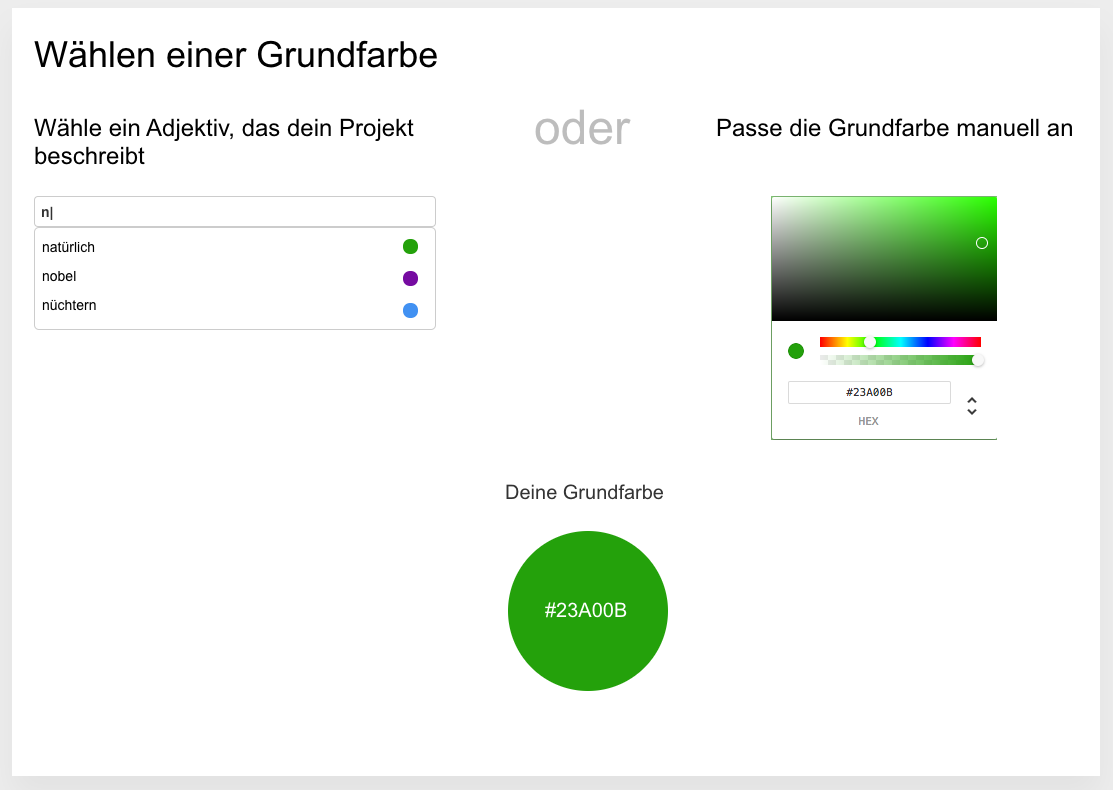
\includegraphics[width=1\textwidth]{images/wireframe-base-color.png}
    \caption{Mögliche Umsetzung der Wahl einer Grundfarbe}
    \label{fig:wire-base-color}
\end{figure}

\subsection{Finden einer Akzentfarbe}
Zum Finden einer Akzentfarbe müssen nun entweder Abstufungen der Grundfarbe, eine zur Grundfarbe komplementäre Farbe oder zwei zur Komplementärefarbe benachbarte Farbtöne gefunden werden

Für die tatsächliche Berechnung im Tool müssen die verwendeten Farben in den HSL-Farbraum (Hue, Saturation, Lightness) konvertiert werden. In diesem Farbraum werden Farbtöne radial auf einem Zylinder angeordnet \cite{joblove1978color}.
Um die Komplementärfarbe einer gegebenen Grundfarbe zu finden, muss also nur die auf dem Kreis gegenüberliegende Farbe gefunden, der Winkel also um 180\degree vergrößert werden. 
Ist die Grundfarbe zum Beispiel ein Grün mit dem HEX-Wert \#23A00B würde dieses zunächst in den HSL-Farbraum konvertiert und die Werte H = 110\degree, S=87\% und L=43\% ergeben. \textit{Saturation} und \textit{Lightness} werden beibehalten, der \textit{Hue}-Wert wird um 180\degree erhöht. Die Komplementärfarbe hat also die Werte  H = 290\degree, S=87\% und L=43\% oder \#AD0ECD.

Soll ein triadisches Farbschema verwendet werden ist, das Vorgehen ähnlich. Hier muss jedoch von der errechenten Komplementärfarbe eine Abstufung im \textit{Hue}-Wert in beide Richtungen gefunden werden. Ein genauer Wert ist schwer zu bestimmen, jedoch liefert eine Abweichung von 30\% in beide Richtungen befreidigende Ergebnisse.\\
Die Komplementärfarbe mit den Werten  H = 290\degree, S=87\% und L=43\% würde also die zwei Abstufungen H = 260\degree, S=100\%, L=50\% und H = 320\degree, S=100\%, L=50\% bzw. \#4E0ECD und \#CD0E8D ergeben.

Um ein monochromatisches Farbschema zu erzeugen, können die \textit{Saturation}- und \textit{Lightness}-Werte verändert werden. Hier bieten sich viele Möglichkeiten, in diesem Beispiel wurden zum Erzeugen von drei Abstufungen zunächst die \textit{Saturation} um 40\% verringert, die \textit{Lightness} um 40\% erhöht und die \textit{Lightness} um 20\% verringert.\\
Die verschiedenen erstellten Farbschemata können Abb. \ref{fig:color-schemes} auf Seite \pageref{fig:color-schemes} entnommen werden. 

\begin{figure}[h]
    \centering
    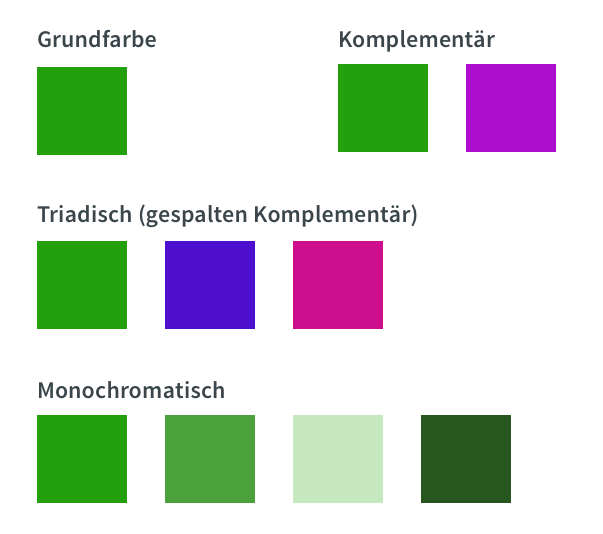
\includegraphics[width=1\textwidth]{images/color-schemes.png}
    \caption{Beispielhaft errechnete Farbpaletten}
    \label{fig:color-schemes}
\end{figure}

Da das Finden der Akzentfarbe ein recht geradliniger Prozess ist fällt es schwer, dem Nutzer hier über die Wahl des von ihm präferierten Farbschemas hinaus viel Interaktivität zu bieten.

\subsection{Komplettieren der Farbpalette}

Nachdem Grund- und Akzentfarbe gefunden sind, fehlen für eine nutzbare Farbpalette noch Grautöne.  Hier sollte darauf geachtet werden, nicht zu viele Grautöne zu verwenden, die sich nur marginal unterscheiden. In den meisten Fällen sollten 2-3 Grautöne in verschiedenen Abstufungen ausreichend sein.
Als einfachste Methode würde es sich anbieten, neutrale Grautöne ohne andere Farben zu wählen. Welche Grautöne genau genutzt werden muss dabei Subjektiv entschieden werden. Denkbar wären zum Beispiel \#eeeeee und \#666666.

\cite{elizabeth2016simple} erläutert eine andere Methode: Bei dieser Methode wird die Grundfarbe mit in die Grautöne eingearbeitet, was ein harmonischeres Bild erzeugt.  Für die Berechnung dieser Werte muss jedoch auf eine externe Bibliothek zurückgegriffen werden.

Hier sollte der Nutzer viele Freiheiten haben, das Tool sollte lediglich kontrollieren, ob die gewählten Grautöne innerhalb einiger Parameter liegen. So kann zum Beispiel über den \textit{Lightness}-Wert des HSL-Farbraumes überprüft werden, ob sich zwei Grautöne deutlich genug unterscheiden. Ebenso kann über den \textit{Saturation}-Wert sicher gestellt werden, dass die Grautöne nicht zu farbig sind.

%----------------------------------------------------------------------------------------

\section{Android \& iOS}\label{androidios}

Für beide Betriebssyteme liegen Guidelines bezüglich der visuellen Gestaltung, auch im Bezug auf Farben, vor. An diese soll sich auch das Tool halten. Das Tool soll hier aber nicht auf diese Guidelines verweisen oder sie wiederholen, sondern eine interaktive Möglichkeit bieten, auch für diese Plattformen eine Farbpalette zu erstellen.

Die Android Guidelines geben zwar keine zwingenden Farben vor, jedoch bieten sie eine große Vorauswahl an Farben, die verwendet werden können. Alle diese Farben sind mit einem Indikator für die Helligkeit versehen, die Guidelines Empfehlen die Farben mit der Helligkeit 500 als Grundfarbe zu benutzen. Hiervon bilden sich dann hellere und dunklere Varianten, die für andere Elemente verwendet werden.
Die Guidelines stellen außerdem eine Menge von Akzentfarben bereit, die frei mit einer der Grundfarben kombiniert werden können. Die Akzentfarbe sollte vor allem für interaktive Elemente verwendet werden.

Die Empfehlung der Farben, basierend auf Adjektiven, kann für Android-Porojekte weiterhin verwendet werden, jedoch mit einer limitierteren Farbauswahl. Akzentfarben müssen nicht mehr errechnet werden, hier kann dem Nutzer eine Auswahl der spezifizierten Akzentfarben gegeben werden, von der er eine auswählen kann.

Die iOS-Richtlinien sind deutlich weniger konkret. Unter iOS wird Farbe vor allem dafür genutzt, Interaktivität deutlich zu machen. Die guidelines schlagen hier 8 Farben vor, die auch dem Nutzer des Tools zur Auswahl gegeben werden sollten. Das Finden einer Akzentfarbe und von Grautönen entfällt dabei komplett. Das Vorschlagen der Farben auf Basis von Adjektiven wäre aber weiterhin, wenn auch recht limitiert, umsetzbar.


